% mnras_template.tex 
%
% LaTeX template for creating an MNRAS paper
%
% v3.0 released 14 May 2015
% (version numbers match those of mnras.cls)
%
% Copyright (C) Royal Astronomical Society 2015
% Authors:
% Keith T. Smith (Royal Astronomical Society)

% Change log
%
% v3.0 May 2015
%    Renamed to match the new package name
%    Version number matches mnras.cls
%    A few minor tweaks to wording
% v1.0 September 2013
%    Beta testing only - never publicly released
%    First version: a simple (ish) template for creating an MNRAS paper

%%%%%%%%%%%%%%%%%%%%%%%%%%%%%%%%%%%%%%%%%%%%%%%%%%
% Basic setup. Most papers should leave these options alone.
\documentclass[fleqn,usenatbib]{mnras}

% MNRAS is set in Times font. If you don't have this installed (most LaTeX
% installations will be fine) or prefer the old Computer Modern fonts, comment
% out the following line
\usepackage{newtxtext,newtxmath}
% Depending on your LaTeX fonts installation, you might get better results with one of these:
%\usepackage{mathptmx}
%\usepackage{txfonts}

% Use vector fonts, so it zooms properly in on-screen viewing software
% Don't change these lines unless you know what you are doing
\usepackage[T1]{fontenc}

% Allow "Thomas van Noord" and "Simon de Laguarde" and alike to be sorted by "N" and "L" etc. in the bibliography.
% Write the name in the bibliography as "\VAN{Noord}{Van}{van} Noord, Thomas"
\DeclareRobustCommand{\VAN}[3]{#2}
\let\VANthebibliography\thebibliography
\def\thebibliography{\DeclareRobustCommand{\VAN}[3]{##3}\VANthebibliography}


%%%%% AUTHORS - PLACE YOUR OWN PACKAGES HERE %%%%%

% Only include extra packages if you really need them. Common packages are:
\usepackage{graphicx}	% Including figure files
\usepackage{amsmath}	% Advanced maths commands
% \usepackage{amssymb}	% Extra maths symbols
\let\Bbbk\relax
\usepackage{amssymb}  % Extra maths symbols
\usepackage{xcolor}
\usepackage{multirow}
% \usepackage{subfig}
\usepackage{caption}
\usepackage{subcaption}

\usepackage[]{booktabs}

%%%%%%%%%%%%%%%%%%%%%%%%%%%%%%%%%%%%%%%%%%%%%%%%%%

%%%%% AUTHORS - PLACE YOUR OWN COMMANDS HERE %%%%%

% Please keep new commands to a minimum, and use \newcommand not \def to avoid
% overwriting existing commands. Example:
%\newcommand{\pcm}{\,cm$^{-2}$}	% per cm-squared

% Please keep new commands to a minimum, and use \newcommand not \def to avoid
% overwriting existing commands. Example:
%\newcommand{\pcm}{\,cm$^{-2}$} % per cm-squared
\graphicspath{{figures}}
% Define prospector as a code type font
\newcommand{\pros}{{\tt \textsc{Prospector}}}
\newcommand{\magp}{{\tt \textsc{Magphys}}}
\newcommand{\cig}{{\tt \textsc{Cigale}}}
\newcommand{\afit}{{\tt \textsc{AGNfitter}}}
\newcommand{\bagp}{{\tt \textsc{Bagpipes}}}
\newcommand{\py}{{\tt \textsc{python}}}
\newcommand{\emcee}{{\tt \textsc{emcee}}}
\newcommand{\dynesty}{{\tt \textsc{Dynesty}}}
\newcommand{\fsps}{{\tt \textsc{FSPS}}}
\newcommand{\tsu}{\textsuperscript}
\newcommand{\tsc}{\textsubscript}

\definecolor{sdasgreen}{RGB}{10, 120, 60}
%%%%%%%%%%%%%%%%%%%%%%%%%%%%%%%%%%%%%%%%%%%%%%%%%%

%%%%%%%%%%%%%%%%%%% TITLE PAGE %%%%%%%%%%%%%%%%%%%

% Title of the paper, and the short title which is used in the headers.
% Keep the title short and informative.
\title[LoTSS galaxy classification with spectra]{LoTSS galaxy classification pro max ultra -- using photometry and spectra}

% The list of authors, and the short list which is used in the headers.
% If you need two or more lines of authors, add an extra line using \newauthor
% \author[S. Das et al.]{
% Soumyadeep Das,$^{1}$\thanks{E-mail: s.das2@herts.ac.uk}
% Marina I. Arnaudova,$^{1}$
% Daniel J. B. Smith,$^{1}$
% Friends and Foes
% \\
% % List of institutions
% $^{1}$Centre for Astrophysics Research, University of Hertfordshire, Hatfield, AL10 9AB, UK.\\
% }

\author[Soumyadeep Das et al.]{Soumyadeep Das$^{1}$\thanks{E-mail: soumyadeep.das.m44@gmail.com},
Daniel J. B. Smith$^{1}$, Marina I. Arnaudova$^{1}$
 \vspace{0.4cm}\\\\ 
 $^{1}$Centre for Astrophysics Research, University of Hertfordshire, Hatfield, AL10 9AB, UK \\ 
}


% These dates will be filled out by the publisher
\date{Accepted XXX. Received YYY; in original form ZZZ}

% Enter the current year, for the copyright statements etc.
\pubyear{2024}

% Don't change these lines
\begin{document}
\label{firstpage}
\pagerange{\pageref{firstpage}--\pageref{lastpage}}
\maketitle

% Abstract of the paper
\begin{abstract}
This is a simple template for authors to write new MNRAS papers.
The abstract should briefly describe the aims, methods, and main results of the paper.
It should be a single paragraph not more than 250 words (200 words for Letters).
No references should appear in the abstract.
\end{abstract}

% Select between one and six entries from the list of approved keywords.
% Don't make up new ones.
\begin{keywords}
keyword1 -- keyword2 -- keyword3
\end{keywords}

%%%%%%%%%%%%%%%%%%%%%%%%%%%%%%%%%%%%%%%%%%%%%%%%%%

%%%%%%%%%%%%%%%%% BODY OF PAPER %%%%%%%%%%%%%%%%%%

\section{Introduction}
- Talk about the low frequency radio population

- Why is classification needed

- previous efforts -- spectra based, phot based -- 

- this paper -  so talk again about desi and lotss


\section{Data}

\begin{figure}
  {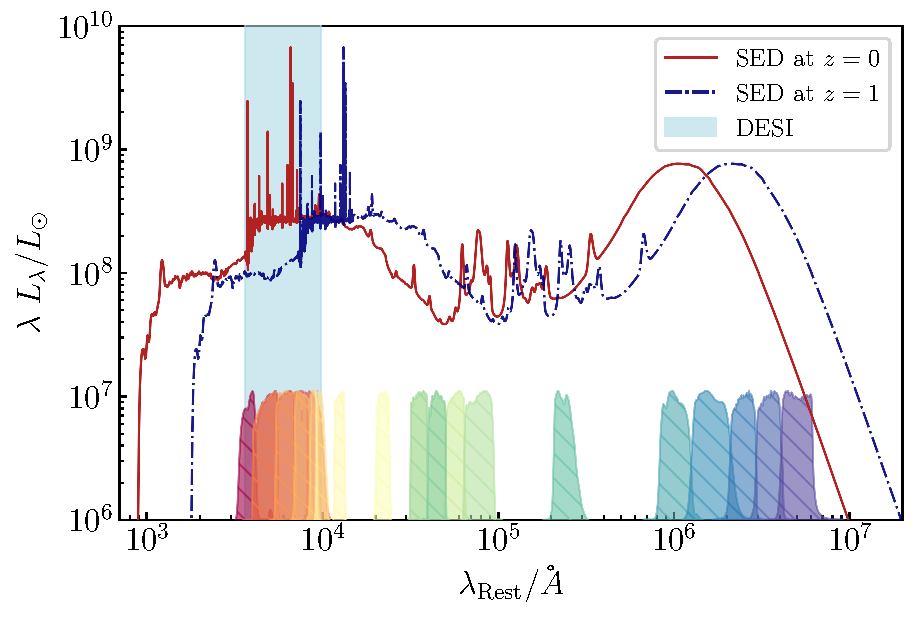
\includegraphics[width=1\columnwidth]{figures/data_coverage.pdf}}
    \caption{(Left panel) 150 MHz radio luminosity coverage of the radio-detected and the $z < 1$ SWIRE-selected source samples used in this work. (Right panel) Histogram showing the number count of sources binned by 150 MHz luminosity for the two data samples. Sources with radio luminosity less than $10^{16}~\mathrm{WHz}^{-1}$ were arbitrarily assigned to the lowest radio luminosity bin.}
    % The inclusion of the radio non-detected sources is often crucial in analyses and provide significant analytical power.  
    \label{fig:filters_jwst_hst}
\end{figure}

\subsection{LoTSS photometry}
ELAIS N1 again...
Describe the filters -- that is sort of there, 

\subsection{DESI Spectra}
Wavelength coverage  - $0.6-5\mu\mathrm{m}$. Three spectral resolutions  - 100, 1000, 2700.

\subsection{Sample selection}
spectra

sample - cuts and all

plot idea - ra dec coverage?? can also add sdss to show how better desi is? Can also include weave to show how better it will be?

\section{Prospector}
\subsection{Model setup}
Do we want to use continuity or bursty? Bursty may be better as it allows a greater degree of freedom.

Do we want to keep c3k library on? What about metallicities? 

\subsection{Parameter estimates}

\section{Results}
\begin{figure*}
  {\includegraphics[width=2\columnwidth]{figures/physical_parameters.pdf}}
    \caption{(Left panel) 150 MHz radio luminosity coverage of the radio-detected and the $z < 1$ SWIRE-selected source samples used in this work. (Right panel) Histogram showing the number count of sources binned by 150 MHz luminosity for the two data samples. Sources with radio luminosity less than $10^{16}~\mathrm{WHz}^{-1}$ were arbitrarily assigned to the lowest radio luminosity bin.}
    % The inclusion of the radio non-detected sources is often crucial in analyses and provide significant analytical power.  
    \label{fig:physical_parameters}
\end{figure*}

\begin{figure*}
  {\includegraphics[width=2\columnwidth]{figures/eta_phot_spec.pdf}}
    \caption{(Left panel) 150 MHz radio luminosity coverage of the radio-detected and the $z < 1$ SWIRE-selected source samples used in this work. (Right panel) Histogram showing the number count of sources binned by 150 MHz luminosity for the two data samples. Sources with radio luminosity less than $10^{16}~\mathrm{WHz}^{-1}$ were arbitrarily assigned to the lowest radio luminosity bin.}
    % The inclusion of the radio non-detected sources is often crucial in analyses and provide significant analytical power.  
    \label{fig:eta_phot_spec}
\end{figure*}


\section{Conclusions}

The last numbered section should briefly summarise what has been done, and describe
the final conclusions which the authors draw from their work.

\section*{Acknowledgements}

The Acknowledgements section is not numbered. Here you can thank helpful
colleagues, acknowledge funding agencies, telescopes and facilities used etc.
Try to keep it short.

%%%%%%%%%%%%%%%%%%%%%%%%%%%%%%%%%%%%%%%%%%%%%%%%%%
\section*{Data Availability}

 
The inclusion of a Data Availability Statement is a requirement for articles published in MNRAS. Data Availability Statements provide a standardised format for readers to understand the availability of data underlying the research results described in the article. The statement may refer to original data generated in the course of the study or to third-party data analysed in the article. The statement should describe and provide means of access, where possible, by linking to the data or providing the required accession numbers for the relevant databases or DOIs.




%%%%%%%%%%%%%%%%%%%% REFERENCES %%%%%%%%%%%%%%%%%%

% The best way to enter references is to use BibTeX:

\bibliographystyle{mnras}
\bibliography{bibfile} % if your bibtex file is called example.bib


% Alternatively you could enter them by hand, like this:
% This method is tedious and prone to error if you have lots of references
%\begin{thebibliography}{99}
%\bibitem[\protect\citeauthoryear{Author}{2012}]{Author2012}
%Author A.~N., 2013, Journal of Improbable Astronomy, 1, 1
%\bibitem[\protect\citeauthoryear{Others}{2013}]{Others2013}
%Others S., 2012, Journal of Interesting Stuff, 17, 198
%\end{thebibliography}

%%%%%%%%%%%%%%%%%%%%%%%%%%%%%%%%%%%%%%%%%%%%%%%%%%

%%%%%%%%%%%%%%%%% APPENDICES %%%%%%%%%%%%%%%%%%%%%

\appendix

\section{Identifying bad fits - phot+spec edition}

\section{Impact of the different data modes on the parameter estimates}
Pacifici like posterior plots

%%%%%%%%%%%%%%%%%%%%%%%%%%%%%%%%%%%%%%%%%%%%%%%%%%


% Don't change these lines
\bsp	% typesetting comment
\label{lastpage}
\end{document}

% End of mnras_template.tex
